\blandscape
\begin{figure}[H]
\centering
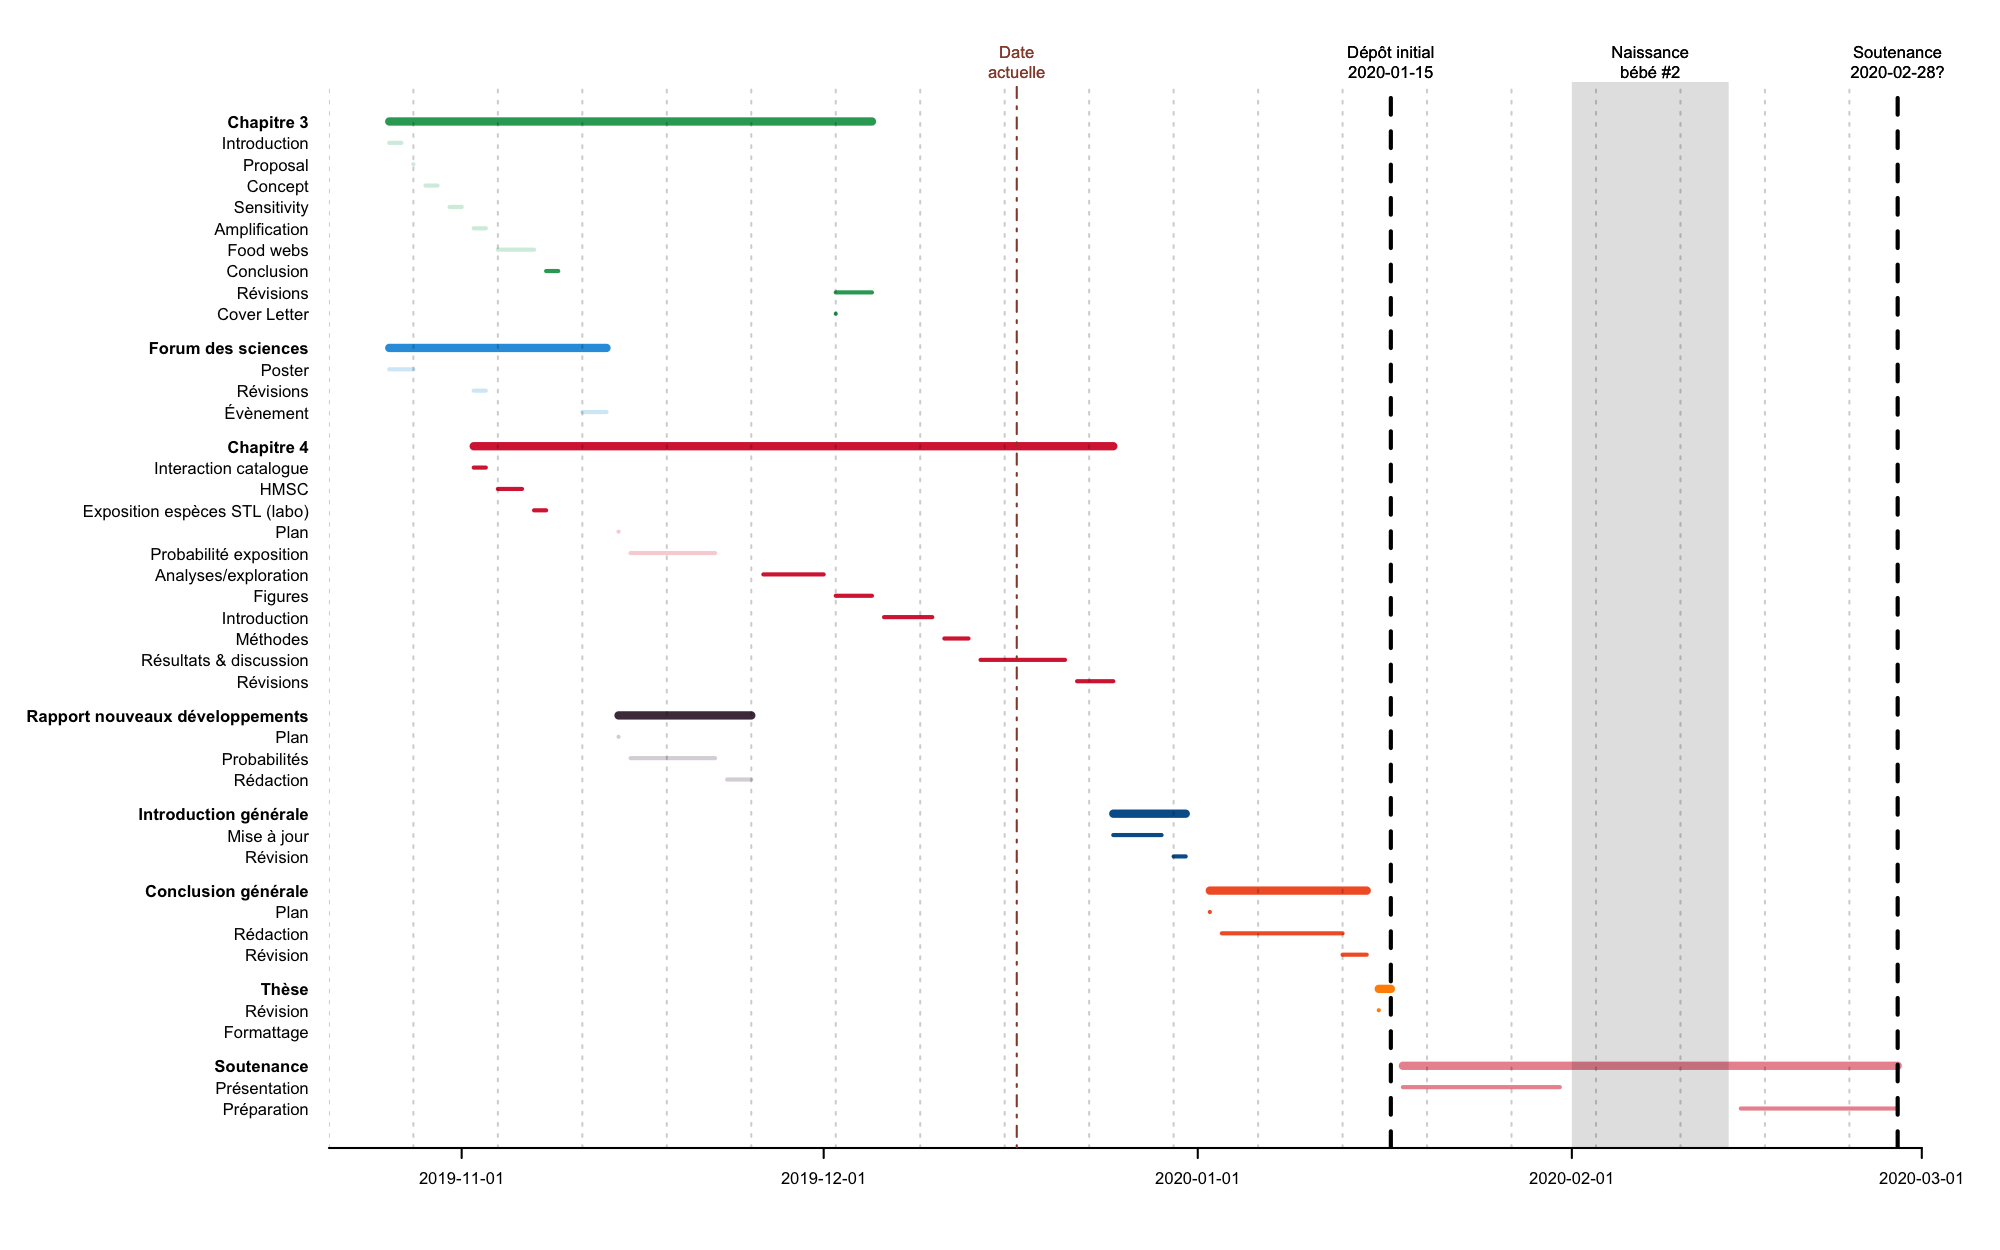
\includegraphics[width=\columnwidth]{./timeline.png}
\label{timeline}
\end{figure}
\elandscape
\newpage

\hypertarget{checklist}{%
\section*{Checklist}\label{checklist}}
\addcontentsline{toc}{section}{Checklist}

\hypertarget{facile}{%
\subsection*{Facile}\label{facile}}
\addcontentsline{toc}{subsection}{Facile}

\begin{itemize}
\tightlist
\item[$\square$]
  Thèse: Dédicace
\item[$\square$]
  Thèse: Remerciements
\item[$\square$]
  Thèse: Avant-propos
\item[$\square$]
  Thèse: Format et numéros de sections
\item[$\boxtimes$]
  Ch1: Références
\item[$\boxtimes$]
  Ch1: Placer figures
\item[$\boxtimes$]
  Ch1: Références figures texte
\item[$\square$]
  Ch1: Tableau 1
\item[$\square$]
  Ch1: Contexte scientifique
\item[$\square$]
  Ch1: Publication associée
\item[$\square$]
  Ch2: Contexte scientifique (Thèse)
\item[$\square$]
  Ch2: Publication associée (Thèse)
\item[$\square$]
  Ch2: Traduction du résumé de l'article publié (Thèse)
\item[$\square$]
  Ch2: Mots clés
\item[$\square$]
  Ch2: Formattage annexe 1
\item[$\square$]
  Ch2: Placer figures
\item[$\square$]
  Ch2: Références figures texte
\item[$\square$]
  Ch3: Contexte scientifique (Thèse)
\item[$\square$]
  Ch3: Publication associée (Thèse)
\item[$\square$]
  Ch3: Traduction du résumé de l'article publié (Thèse)
\item[$\square$]
  Ch3: Mots clés
\item[$\square$]
  Ch3: Formattage annexe 2
\item[$\square$]
  Ch3: Placer figures
\item[$\square$]
  Ch3: Références figures texte
\item[$\square$]
  Ch4: Define pathways
\item[$\boxtimes$]
  Ch4: Conceptual figure formatting + letters
\item[$\square$]
  Ch4: Number of pathways / motifs \& positions
\item[$\square$]
  Ch4: Contexte scientifique (Thèse)
\item[$\square$]
  Ch4: Publication associée (Thèse)
\item[$\square$]
  Ch4: Traduction du résumé de l'article publié (Thèse)
\item[$\square$]
  Ch4: Mots clés
\item[$\square$]
  Ch4: Formattage annexe 3
\item[$\square$]
  Ch4: Statement of authorship
\item[$\square$]
  Ch4: Data accessibility statement
\item[$\square$]
  Ch4: Reviewers
\item[$\square$]
  Ch4: Acknowledgements
\item[$\square$]
  Ch4: References
\item[$\square$]
  Ch5: Contexte scientifique (Thèse)
\item[$\square$]
  Ch5: Publication associée (Thèse)
\item[$\square$]
  Ch5: Traduction du résumé de l'article publié (Thèse)
\item[$\square$]
  Ch5: Mots clés
\item[$\square$]
  Ch5: Formattage annexe 4
\item[$\square$]
  Ch5: Scientific report \textbar{} Science format
\item[$\square$]
  Ch5: Acknowledgements
\item[$\square$]
  CG: Plan conclusion générale
\end{itemize}

\hypertarget{moyen}{%
\subsection*{Moyen}\label{moyen}}
\addcontentsline{toc}{subsection}{Moyen}

\begin{itemize}
\tightlist
\item[$\square$]
  Thèse: Résumé de la thèse (fr)
\item[$\square$]
  Thèse: Résumé de la thèse (en)
\item[$\square$]
  IG: Réviser introduction générale
\item[$\square$]
  IG: Mettre à jour les objectifs de la thèse
\item[$\square$]
  IG: Diviser la thèse en 3: stresseurs, communautés, impacts cumulés
\item[$\boxtimes$]
  Ch4: Figure densités
\item[$\square$]
  Ch4: Graph units
\item[$\square$]
  Ch4: Cover letter and novelty statement
\item[$\square$]
  CG: Brainstorm
\end{itemize}

\hypertarget{difficile}{%
\subsection*{Difficile}\label{difficile}}
\addcontentsline{toc}{subsection}{Difficile}

\begin{itemize}
\tightlist
\item[$\square$]
  IG: Mettre à jour avec la littérature récente
\item[$\square$]
  Ch4: Discussion
\item[$\square$]
  Ch4: Lecture articles
\item[$\square$]
  Ch5: Données environnementales
\item[$\square$]
  Ch5: HMSC
\item[$\square$]
  Ch5: iEat
\item[$\square$]
  Ch5: Analyses CI communautés
\item[$\square$]
  Ch5: Abstract
\item[$\square$]
  Ch5: Introduction
\item[$\square$]
  Ch5: annexe 4
\item[$\square$]
  Ch5: Methods
\item[$\square$]
  Ch5: Results
\item[$\square$]
  Ch5: Discussion
\item[$\square$]
  Ch5: Figures
\item[$\square$]
  CG: Description et présentation des analyses globales
\item[$\square$]
  CG: Retour sur les principaux résultats de la thèse
\item[$\square$]
  CG: Perspectives
\end{itemize}

\hypertarget{guxe9nuxe9ral}{%
\subsection*{Général}\label{guxe9nuxe9ral}}
\addcontentsline{toc}{subsection}{Général}

\begin{itemize}
\tightlist
\item[$\square$]
  Composition jury
\item[$\square$]
  Dédicace(?)
\item[$\square$]
  Remerciements
\item[$\square$]
  Avant-propos
\item[$\square$]
  Résumé de la thèse (fr)
\item[$\square$]
  Résumé de la thèse (en)
\item[$\square$]
  Liste des abbréviations(?)
\item[$\square$]
  Introduction générale
\item[$\square$]
  Chapitre 1: Naturaliste Canadien - Cumulative impacts in the
  St.~Lawrence
\item[$\square$]
  Chapitre 2: Frontiers in Marine Sciences - Drivers
\item[$\square$]
  Chapitre 3: Milieu \& Vie - iEat
\item[$\square$]
  Chapitre 4: Ecology Letters paper - Of food webs and multiple
  disturbances
\item[$\square$]
  Chapitre 5: Cumulative impacts on food webs
\item[$\square$]
  Conclusion générale
\item[$\square$]
  Annexe 1: Supplementary information chapitre 2
\item[$\square$]
  Annexe 2: Supplementary information chapitre 3
\item[$\square$]
  Annexe 3: Supplementary information chapitre 4
\item[$\square$]
  Annexe 4: Supplementary information chapitre 5
\item[$\square$]
  References
\end{itemize}

\hypertarget{liste-articles-uxe0-lire}{%
\subsection*{Liste articles à lire}\label{liste-articles-uxe0-lire}}
\addcontentsline{toc}{subsection}{Liste articles à lire}

\begin{itemize}
\tightlist
\item[$\square$]
  \citet{bousquet2019} Cod northern St.~Lawrence
\item[$\square$]
  \citet{bundy2005} Cod northern St.~Lawrence
\item[$\square$]
  \citet{burns2014} Perturbations direct \& indirect effects
\item[$\square$]
  \citet{frank2005} Cod
\item[$\square$]
  \citet{jackson2001} Overfishing
\item[$\square$]
  \citet{myers2003} Depletion of fish
\item[$\square$]
  \citet{ogorman2009}
\item[$\square$]
  \citet{ogorman2010}
\item[$\square$]
  \citet{ogorman2012}
\item[$\square$]
  \citet{ogorman2019}
\item[$\square$]
  \citet{worm2002}
\item[$\square$]
  \citet{zhang2019}
\item[$\square$]
  \citet{mcdonaldmadden2016} food webs \& conservation
\item[$\square$]
  \citet{abdalaroberts2019}
\item[$\square$]
  \citet{gillaranz2016}
\item[$\square$]
  \citet{gillaranz2017}
\item[$\square$]
  \citet{dupontavice2019}
\end{itemize}

\hypertarget{composition-jury}{%
\subsection*{Composition jury}\label{composition-jury}}
\addcontentsline{toc}{subsection}{Composition jury}

\begin{itemize}
\tightlist
\item
  Isabelle Côté
\item
  Guy Woodward
\item
  Daniel Stouffer
\item
  Nathalie Ban
\item
  Kevin McCann
\item
  Tasman Crowe
\end{itemize}

\hypertarget{introduction-guxe9nuxe9rale}{%
\subsection*{Introduction générale}\label{introduction-guxe9nuxe9rale}}
\addcontentsline{toc}{subsection}{Introduction générale}

\begin{itemize}
\tightlist
\item[$\square$]
  Réviser introduction générale
\item[$\square$]
  Mettre à jour avec la littérature récente
\item[$\square$]
  Mettre à jour les objectifs de la thèse
\item[$\square$]
  Diviser la thèse en 3: stresseurs, communautés, impacts cumulés
\end{itemize}

\hypertarget{chapitre-1}{%
\subsection*{Chapitre 1}\label{chapitre-1}}
\addcontentsline{toc}{subsection}{Chapitre 1}

\begin{itemize}
\tightlist
\item[$\boxtimes$]
  Retranscrire article
\item[$\square$]
  Contexte scientifique (Thèse)
\item[$\square$]
  Publication associée (Thèse)
\item[$\square$]
  Traduction du résumé de l'article publié (Thèse)
\item[$\boxtimes$]
  Références
\item[$\boxtimes$]
  Table
\item[$\boxtimes$]
  Figures
\item[$\boxtimes$]
  Box
\item[$\square$]
  keywords
\end{itemize}

\hypertarget{chapitre-2}{%
\subsection*{Chapitre 2}\label{chapitre-2}}
\addcontentsline{toc}{subsection}{Chapitre 2}

\begin{itemize}
\tightlist
\item[$\square$]
  Retranscrire article
\item[$\square$]
  Contexte scientifique (Thèse)
\item[$\square$]
  Publication associée (Thèse)
\item[$\square$]
  Traduction du résumé de l'article publié (Thèse)
\item[$\boxtimes$]
  Références
\item[$\boxtimes$]
  Table
\item[$\boxtimes$]
  Figures
\item[$\boxtimes$]
  Box
\item[$\square$]
  keywords
\end{itemize}

\hypertarget{chapitre-3}{%
\subsection*{Chapitre 3}\label{chapitre-3}}
\addcontentsline{toc}{subsection}{Chapitre 3}

\begin{itemize}
\tightlist
\item[$\square$]
  Retranscrire article
\item[$\square$]
  Contexte scientifique (Thèse)
\item[$\square$]
  Publication associée (Thèse)
\item[$\square$]
  Traduction du résumé de l'article publié (Thèse)
\item[$\square$]
  Références
\item[$\square$]
  keywords
\item[$\square$]
  Format table in appendice
\end{itemize}

\hypertarget{chapitre-4}{%
\subsection*{Chapitre 4}\label{chapitre-4}}
\addcontentsline{toc}{subsection}{Chapitre 4}

\begin{itemize}
\tightlist
\item[$\square$]
  Contexte scientifique (Thèse)
\item[$\square$]
  Publication associée (Thèse)
\item[$\square$]
  Traduction du résumé de l'article publié (Thèse)
\item[$\boxtimes$]
  Proposal letter Ecology Letters - Ideas and Perspectives
\item[$\square$]
  Cover letter and novelty statement
\item[$\boxtimes$]
  Conflict of interest statement
\item[$\square$]
  Statement of authorship
\item[$\square$]
  Data accessibility statement
\item[$\square$]
  Reviewers
\item[$\boxtimes$]
  Keywords
\item[$\boxtimes$]
  Abstract
\item[$\boxtimes$]
  Introduction
\item[$\boxtimes$]
  Of food webs and multiple disturbances (concept)
\item[$\boxtimes$]
  Simulations
\item[$\square$]
  Sensitivity
\item[$\square$]
  Amplification
\item[$\square$]
  Food web sensitivity \& amplification
\item[$\square$]
  Conclusions
\item[$\square$]
  Acknowledgements
\item[$\square$]
  References
\item[$\boxtimes$]
  Figure 1 - Concept
\item[$\square$]
  Figure 2 - Vulnerability
\item[$\boxtimes$]
  Figure 3 - Position vulnerability
\item[$\boxtimes$]
  Figure 4 - Parameter type
\item[$\boxtimes$]
  Figure 5 - Food web scores table
\item[$\boxtimes$]
  Figure 6 - Species
\item[$\boxtimes$]
  Table S1 - Systems of equations
\item[$\boxtimes$]
  Figure S1 - Score table 2
\item[$\boxtimes$]
  Figure S2 - Score table 3
\item[$\square$]
  Article formatting
\end{itemize}

\hypertarget{chapitre-5}{%
\subsection*{Chapitre 5}\label{chapitre-5}}
\addcontentsline{toc}{subsection}{Chapitre 5}

\begin{itemize}
\tightlist
\item[$\square$]
  Données
\item[$\square$]
  Catalogue interactions
\item[$\square$]
  HMSC
\item[$\square$]
  Plan article
\item[$\square$]
  Article de soumission
\end{itemize}

\hypertarget{conclusion-guxe9nuxe9rale}{%
\subsection*{Conclusion générale}\label{conclusion-guxe9nuxe9rale}}
\addcontentsline{toc}{subsection}{Conclusion générale}

\begin{itemize}
\tightlist
\item[$\square$]
  Plan conclusion générale
\item[$\square$]
  Brainstorm
\item[$\square$]
  Description et présentation des analyses globales
\item[$\square$]
  Retour sur les principaux résultats de la thèse
\item[$\square$]
  Perspectives
\end{itemize}
